\documentclass[crop,tikz,convert={outext=.svg,command=\unexpanded{pdf2svg \infile\space\outfile}},multi=false]{standalone}[2012/04/13]
\usepackage{tikz}
\usepackage{pgfplots}

\usetikzlibrary{arrows,shapes,positioning}
\usetikzlibrary{automata, positioning}

\begin{document}
	
	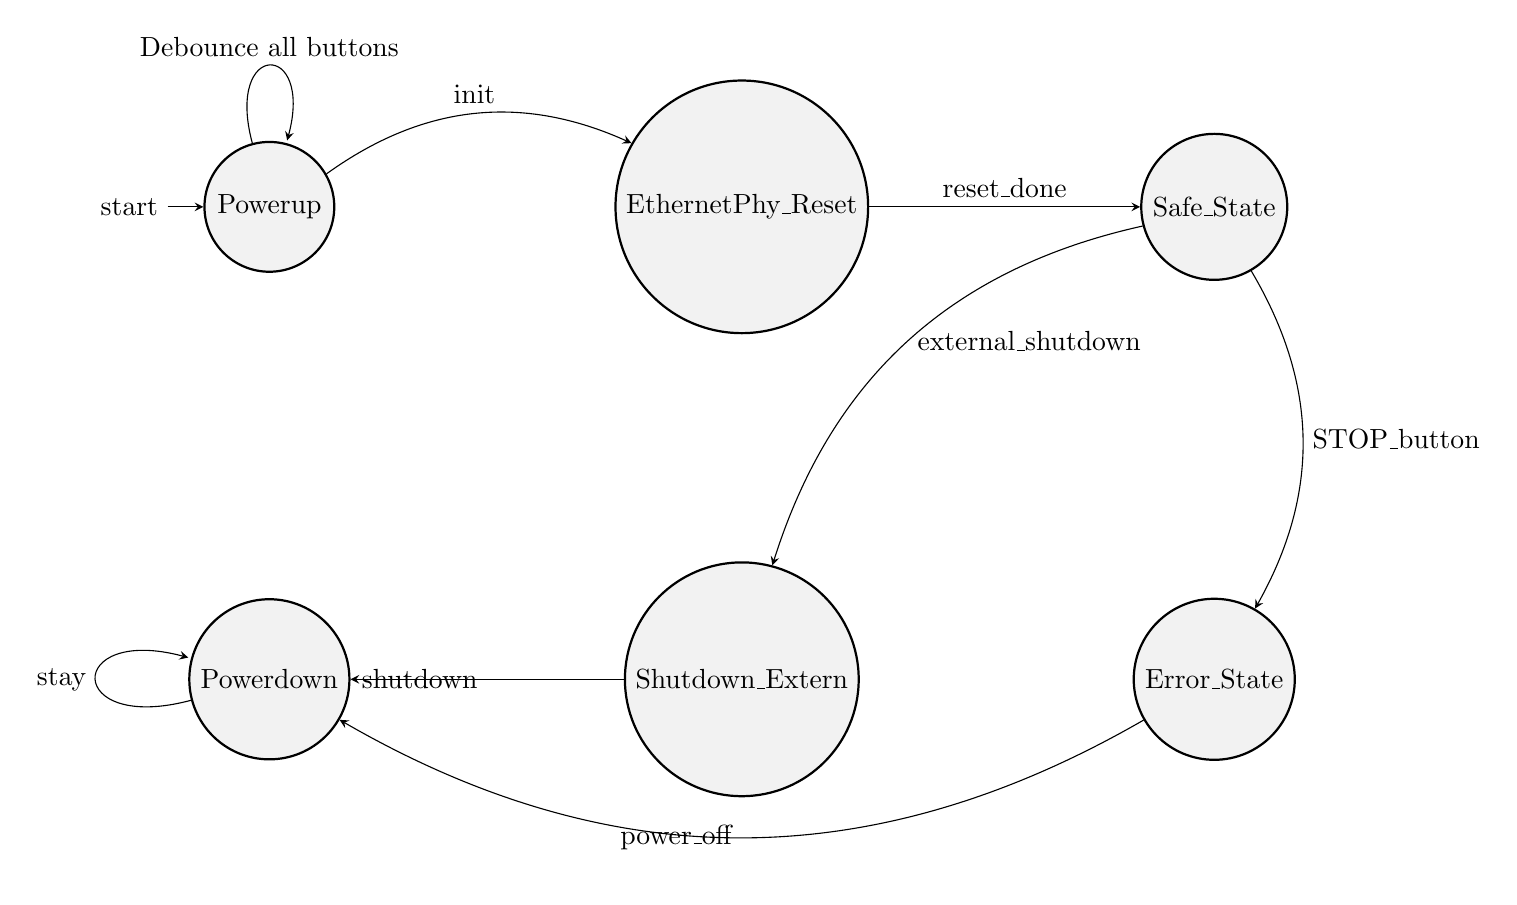
\begin{tikzpicture}[->, >=stealth, node distance=6cm, every state/.style={thick, fill=gray!10}]
		% Define states
		\node[state, initial] (Powerup) {Powerup};
		\node[state, right of=Powerup] (EthernetPhy_Reset) {EthernetPhy\_Reset};
		\node[state, right of=EthernetPhy_Reset] (Safe_State) {Safe\_State};
		\node[state, below of=Safe_State] (Error_State) {Error\_State};
		\node[state, below of=EthernetPhy_Reset] (Shutdown_Extern) {Shutdown\_Extern};
		\node[state, left of=Shutdown_Extern] (Powerdown) {Powerdown};
		
		% Define transitions
		\path 
		(Powerup) edge[loop above] node[above] {Debounce all buttons} (Powerup)
		(Powerup) edge[bend left] node[above] {init} (EthernetPhy_Reset)
		(EthernetPhy_Reset) edge node[above] {reset\_done} (Safe_State)
		(Safe_State) edge[bend left] node[right] {STOP\_button} (Error_State)
		(Error_State) edge[bend left] node[left] {power\_off} (Powerdown)
		(Shutdown_Extern) edge node[left] {shutdown} (Powerdown)
		(Safe_State) edge[bend right] node[right] {external\_shutdown} (Shutdown_Extern)
		(Powerdown) edge[loop left] node[left] {stay} (Powerdown);
	\end{tikzpicture}
	
\end{document}